\documentclass[../../master_thesis_np.tex]{subfiles}
\graphicspath{{./imgs/}}

\begin{document}
\chapter[Interaction Implementation]{Implementation of interactions in simulations}
\label{chap:int_impl}
	\section{Previous Developments}
	All the code work in this project is written in\ \julia programming language, built on top of an existing code written and used in {\color{blue} MRLAB}. The existing code base was able to perform simulations of systems of active brownian particles in 2D with closed, periodic or open boundary conditions featuring several confinement shapes. The only interaction which was featured in the model was a steric hard sphere correction, which is enough to study clustering and motility-induced phase  separation, as well as boundary accumulation phenomena. The hardsphere correction follows algorithm \ref{alg:hardsphere} according to \parencite{callegari_numerical_2019}.
	\parencite{martin-gomez_collective_2018}

	\begin{algorithm}[htp]
		\caption{The hard sphere correction algorithm} \label{alg:hardsphere}	
		\begin{algorithmic}[1]
			\ForAll{couples of particles $\{i, j\}$}
			\State{$d_{i,j} \gets d(\mathbf{r}_{i}, \mathbf{r}_{j})$} \Comment{$d\left(\cdot,\cdot \right)$ is the Euclidean distance}

			\State{$\mathbf{n}_{i,j} = \left(\mathbf{r}_{i}-\mathbf{r}_{j}\right)/d_{i,j}$}
			\If{$d_{i,j} < 2R$}\Comment{$R$ is the particles' radius}
			\State{$\mathbf{r}_i \gets \mathbf{r}_i - \mathbf{n}_{i,j}d_{i,j}/2$}
			\State{$\mathbf{r}_j \gets \mathbf{r}_i - \mathbf{n}_{j,i}d_{i,j}/2$}
			\EndIf
			\EndFor
		\end{algorithmic}
		\end{algorithm}

		\begin{figure}[htp]
			\centering
			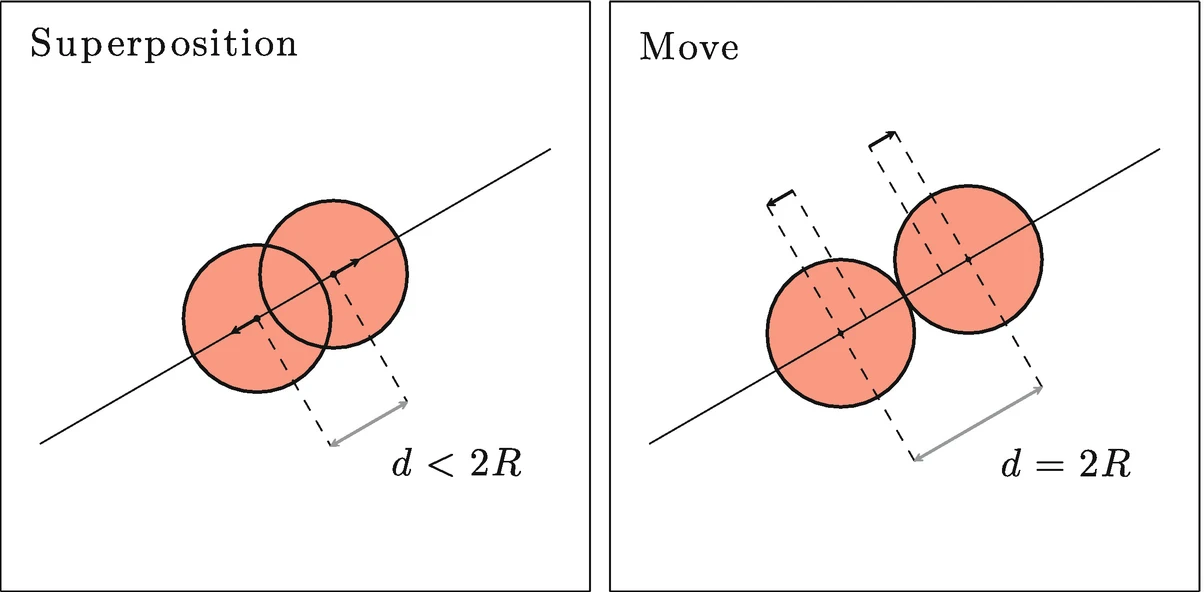
\includegraphics[width = 0.7\textwidth]{callegari_volpe_2019_hardsphere.png}
			\label{fig:hardsphere}
			\caption{{\small \fullcite{callegari_numerical_2019}}}
		\end{figure}

	Clearly, being a $O(n^2)$ algorithm, this kind of correction can become computationally heavy, especially for high density systems, as well as high velocity systems, where clustering is more likely.
	
	Since the original code base was designed to study ABPs in confinements rather than in periodic boundary conditions, this interaction could not take periodicity into account leading to possible superpositions at the boundaries.

	\section{Steric Interactions}
	\subsection{All to All}
	\subsection{Range}
	\section{Aligning Interactions}

\end{document}